\newcommand{\svcourse}{CST Part IA: Software Engineering and Security}
\newcommand{\svnumber}{1}
\newcommand{\svvenue}{Microsoft Teams}
\newcommand{\svdate}{2022-05-11}
\newcommand{\svtime}{15:00}
\newcommand{\svuploadkey}{CBd13xmL7PC1zqhNIoLdTiYUBnxZhzRAtJxv/ytRdM1r7qIfwMsxeVwM/pPcIo8l}

\newcommand{\svrname}{Dr Sam Ainsworth}
\newcommand{\jkfside}{oneside}
\newcommand{\jkfhanded}{yes}

\newcommand{\studentname}{Harry Langford}
\newcommand{\studentemail}{hjel2@cam.ac.uk}


\documentclass[10pt,\jkfside,a4paper]{article}

\usepackage{float}
\usepackage{tikz}
\usepackage[utf8]{inputenc}
\usepackage[T1]{fontenc}
\usepackage{graphicx}
\usetikzlibrary{arrows,shapes,automata,petri,positioning,calc}

\tikzset{
	node distance=0.7cm,
    place/.style={
        circle,
        thick,
        draw=black,
        fill=lightgray!20,
        minimum size=7mm,
    },
        state/.style={
        circle,
        thick,
        minimum size=7mm,
    },
    place2/.style={
        circle,
        thick,
        draw=black,
        fill=lightgray!20,
        minimum size=10mm,
    },
    place3/.style={
        circle,
        thick,
        draw=black,
        fill=lightgray!20,
        minimum size=20mm,
    }
}

% DO NOT add \usepackage commands here.  Place any custom commands
% into your SV work files.  Anything in the template directory is
% likely to be overwritten!

\usepackage{fancyhdr}

\usepackage{lastpage}       % ``n of m'' page numbering
\usepackage{lscape}         % Makes landscape easier

\usepackage{verbatim}       % Verbatim blocks
\usepackage{listings}       % Source code listings
\usepackage{graphicx}
\usepackage{float}
\usepackage{epsfig}         % Embed encapsulated postscript
\usepackage{array}          % Array environment
\usepackage{qrcode}         % QR codes
\usepackage{enumitem}       % Required by Tom Johnson's exam question header

\usepackage{hhline}         % Horizontal lines in tables
\usepackage{siunitx}        % Correct spacing of units
\usepackage{amsmath}        % American Mathematical Society
\usepackage{amssymb}        % Maths symbols
\usepackage{amsthm}         % Theorems

\usepackage{ifthen}         % Conditional processing in tex

\usepackage[top=3cm,
            bottom=3cm,
            inner=2cm,
            outer=5cm]{geometry}

% PDF metadata + URL formatting
\usepackage[
            pdfauthor={\studentname},
            pdftitle={\svcourse, SV \svnumber},
            pdfsubject={},
            pdfkeywords={9d2547b00aba40b58fa0378774f72ee6},
            pdfproducer={},
            pdfcreator={},
            hidelinks]{hyperref}

\renewcommand{\headrulewidth}{0.4pt}
\renewcommand{\footrulewidth}{0.4pt}
\fancyheadoffset[LO,LE,RO,RE]{0pt}
\fancyfootoffset[LO,LE,RO,RE]{0pt}
\pagestyle{fancy}
\fancyhead{}
\fancyhead[LO,RE]{{\bfseries \studentname}\\\studentemail}
\fancyhead[RO,LE]{{\bfseries \svcourse, SV~\svnumber}\\\svdate\ \svtime, \svvenue}
\fancyfoot{}
\fancyfoot[LO,RE]{For: \svrname}
\fancyfoot[RO,LE]{\today\hspace{1cm}\thepage\ / \pageref{LastPage}}
\fancyfoot[C]{\qrcode[height=0.8cm]{\svuploadkey}}
\setlength{\headheight}{22.55pt}


\ifthenelse{\equal{\jkfside}{oneside}}{

 \ifthenelse{\equal{\jkfhanded}{left}}{
  % 1. Left-handed marker, one-sided printing or e-marking, use oneside and...
  \evensidemargin=\oddsidemargin
  \oddsidemargin=73pt
  \setlength{\marginparwidth}{111pt}
  \setlength{\marginparsep}{-\marginparsep}
  \addtolength{\marginparsep}{-\textwidth}
  \addtolength{\marginparsep}{-\marginparwidth}
 }{
  % 2. Right-handed marker, one-sided printing or e-marking, use oneside.
  \setlength{\marginparwidth}{111pt}
 }

}{
 % 3. Alternating margins, two-sided printing, use twoside.
}


\setlength{\parindent}{0em}
\addtolength{\parskip}{1ex}

% Exam question headings, labels and sensible layout (courtesy of Tom Johnson)
\setlist{parsep=\parskip, listparindent=\parindent}
\newcommand{\examhead}[3]{\section{#1 Paper #2 Question #3}}
\newenvironment{examquestion}[3]{
\examhead{#1}{#2}{#3}\setlist[enumerate, 1]{label=(\alph*)}\setlist[enumerate, 2]{label=(\roman*)}
\marginpar{\href{https://www.cl.cam.ac.uk/teaching/exams/pastpapers/y#1p#2q#3.pdf}{\qrcode{https://www.cl.cam.ac.uk/teaching/exams/pastpapers/y#1p#2q#3.pdf}}}
\marginpar{\footnotesize \href{https://www.cl.cam.ac.uk/teaching/exams/pastpapers/y#1p#2q#3.pdf}{https://www.cl.cam.ac.uk/\\teaching/exams/pastpapers/\\y#1p#2q#3.pdf}}
}{}


\begin{document}

\section{Example Sheet 4}

\begin{enumerate}

\item Draw the state space diagram for this Markov chain.

\begin{lstlisting}[language=Python]
def rw():
	MAX_STATE = 9
	x = 0
	while True:
		yield x
		d = np.random.choice([-1, 0, 1], p=[0.25, 0.5, 0.25])
		x = min(MAX_STATE, max(0, x + d))
\end{lstlisting}

\begin{center}
\begin{tikzpicture}
\node [state, place] (node0) {0};
\node [state, place] (node1) [right = of node0] {1};
\node [state, place] (node2) [right = of node1] {2};
\node [state, place] (node3) [right = of node2] {3};
\node [state, place] (node4) [right = of node3] {4};
\node [state, place] (node5) [right = of node4] {5};
\node [state, place] (node6) [right = of node5] {6};
\node [state, place] (node7) [right = of node6] {7};
\node [state, place] (node8) [right = of node7] {8};
\node [state, place] (node9) [right = of node8] {9};
\path [->] (node0) edge [loop left] node {$\frac{3}{4}$} ();
\path [->] (node0) edge [bend left] node[above] {$\frac{1}{4}$} (node1);
\path [->] (node1) edge [bend left] node[below] {$\frac{1}{4}$} (node0);
\path [->] (node1) edge [bend left] node[above] {$\frac{1}{4}$} (node2);
\path [->] (node2) edge [bend left] node[below] {$\frac{1}{4}$} (node1);
\path [->] (node2) edge [bend left] node[above] {$\frac{1}{4}$} (node3);
\path [->] (node3) edge [bend left] node[below] {$\frac{1}{4}$} (node2);
\path [->] (node3) edge [bend left] node[above] {$\frac{1}{4}$} (node4);
\path [->] (node4) edge [bend left] node[below] {$\frac{1}{4}$} (node3);
\path [->] (node4) edge [bend left] node[above] {$\frac{1}{4}$} (node5);
\path [->] (node5) edge [bend left] node[below] {$\frac{1}{4}$} (node4);
\path [->] (node5) edge [bend left] node[above] {$\frac{1}{4}$} (node6);
\path [->] (node6) edge [bend left] node[below] {$\frac{1}{4}$} (node5);
\path [->] (node6) edge [bend left] node[above] {$\frac{1}{4}$} (node7);
\path [->] (node7) edge [bend left] node[below] {$\frac{1}{4}$} (node6);
\path [->] (node7) edge [bend left] node[above] {$\frac{1}{4}$} (node8);
\path [->] (node8) edge [bend left] node[below] {$\frac{1}{4}$} (node7);
\path [->] (node8) edge [bend left] node[above] {$\frac{1}{4}$} (node9);
\path [->] (node9) edge [bend left] node[below] {$\frac{1}{4}$} (node8);
\path [->] (node9) edge [loop right] node {$\frac{3}{4}$} ();
\path [->] (node1) edge [loop above] node {$\frac{1}{2}$} ();
\path [->] (node2) edge [loop above] node {$\frac{1}{2}$} ();
\path [->] (node3) edge [loop above] node {$\frac{1}{2}$} ();
\path [->] (node4) edge [loop above] node {$\frac{1}{2}$} ();
\path [->] (node5) edge [loop above] node {$\frac{1}{2}$} ();
\path [->] (node6) edge [loop above] node {$\frac{1}{2}$} ();
\path [->] (node7) edge [loop above] node {$\frac{1}{2}$} ();
\path [->] (node8) edge [loop above] node {$\frac{1}{2}$} ();
\end{tikzpicture}
\end{center}

\item For the Cambridge weather simulator, example 10.2.1 in the lecture
notes, show that

\[
\mathbb{P}(X_3 = r \ | \ X_0 = g) = \sum^{}_{x_1, x_2}
P_{g x_1}P_{x_1 x_2}P_{x_2 r}
\]

\[
\begin{split}
P(X=r \ | \ X_0 = g)
&= P^3_{g, r} \\
&= \sum_{x_1, x_2}  P_{g x_1} P_{x_1 x_2} P_{x_2 r} \\
\end{split}
\]

\item here is the state space diagram for a Markov chain with a state space
\{0, 1, \dots, $N$\}. States 0 and $N$ are absorbing states. at any other
state $x$ we jump to $x - 1$ with probability $\alpha$ and to $x + 1$ with
probability $\beta$. Assume $\alpha > 0$ and $\beta > 0$ and $\alpha + \beta
\leq 1$. Let $h_x = \mathbb{P}(\text{hit} \ 0 \ | \ \text{start at} \ x)$.

\begin{itemize}

\item For $N = 3$, calculate $h_x$ for all $x \in \{0, 1, 2, 3\}$.

\begin{align*}
h_0 &= 1 & h_1 &= \beta h_0 + (1 - \alpha - \beta) h_1 + \alpha h_2 \\
h_2 &= \beta h_1 + (1 - \alpha - \beta) h_2 + \alpha h_3 & h_3 &= 0 \\
\end{align*}
\[
\begin{split}
h_1 &= \beta h_0 + (1 - \alpha - \beta) h_1 + \alpha h_2 \\
(\alpha + \beta)h_1 &= \beta + \alpha h_2 \\
h_2 &= \beta h_1 + (1 - \alpha - \beta) h_2 + \alpha h_3 \\
(\alpha + \beta)h_2 &= \beta h_1 \\
(\alpha + \beta)h_1 &= \beta + \frac{\alpha \beta}{\alpha + \beta} h_1 \\
h_1 &= \frac{\beta(\alpha + \beta)}{\alpha^2 + \alpha \beta + \beta^2} \\
h_2 &= \frac{\alpha\beta}{\alpha^2 + \alpha \beta + \beta^2} \\
\end{split}
\]

\begin{align*}
h_0 &= 1
&
h_1 &= \frac{\beta(\alpha + \beta)}{\alpha^2 + \alpha \beta + \beta^2}
\\
h_2 &= \frac{\alpha\beta}{\alpha^2 + \alpha \beta + \beta^2}
&
h_3 &= 0
\end{align*}

\item For arbitrary $N$, give code to compute the vector $[h_0, h_1, \dots,
h_n]$.

\begin{lstlisting}[language=Python, mathescape=true]
P = np.zeros((N + 1, N + 1))
P[np.arange(1, N), np.arange(N - 1)] = $\beta$
P[np.arange(1, N), np.arange(1, N)] = 1 - $\alpha$ - $\beta$
P[np.arange(1, N), np.arange(2, N + 1)] = $\alpha$
P[0, 0] = 1
P[N, N] = 1
conditions = np.zeros((2, N + 1))
conditions[0, 0] = 1
conditions[-1, -1] = 1
mat = np.concatenate((P - np.eye(N + 1), conditions))
target = np.zeros(N + 3)
target[-2] = 1
np.linalg.lstsq(mat, target, rcond=None)
\end{lstlisting}

\end{itemize}

\item Consider a random walk on the vertices of this undirected graph as
follows: each timestep we take one of the edges chosen at random, each edge
from our current vertex equally likely. Find the stationary distribution.

The stationary distribution is as follows:
\[
\begin{pmatrix}
\frac{1}{8}, &
\frac{3}{8}, &
\frac{2}{8}, &
\frac{2}{8}
\end{pmatrix}
\]

We can calculate this by either applying the standard result for the
stationary distribution of a random walk on an undirected graph -- $\pi_i$ is
the number of edges $i$ has divided by twice the total number of edges.

Or we can use the code below:
\begin{lstlisting}[language=Python]
P = np.array([
	[0, 1, 0, 0],
	[1/3, 0, 1/3, 1/3],
	[0, 1/2, 0, 1/2],
	[0, 1/2, 1/2, 0],
])
mat = np.concatenate((P.transpose() - np.eye(4), np.ones((1, 4))))
np.linalg.lstsq(mat,[0, 0, 0, 0, 1], rcond=None)
\end{lstlisting}

\item Let $X_n$ be a mean-reverting random walk,

\[
X_{n + 1} = \mu + \lambda(X_n - \mu) + \mathcal{N}(0, \sigma^2) \ \ \
\text{where} \ \ \ -1 < \lambda < 1
\]

The stationary distribution for this process is a normal distribution. Find
its parameters.

Since the distribution is stationary: $\mathbb{E}(X_{n+1}) = \mathbb{E}(X_n)$
\[
\begin{split}
\mathbb{E}(X_n) &= \mathbb{E}(X_{n+1}) \\
\mathbb{E}(X_n) &= \mathbb{E}(\mu + \lambda(X_n - \mu) + \mathcal{N}(0,
\sigma^2)) \\
\mathbb{E}(X_n) &= \mu + \lambda(\mathbb{E}(X_n) - \mu) + 0 \\
(1 - \lambda)\mathbb{E}(X_n) &= (1 - \lambda)\mu \\
\mathbb{E}(X_n) &= \mu \\
\end{split}
\]
Therefore if $X_n$ is normally distributed then it has mean $\mu$.

Since the distribution is stationary, $\mathbb{E}(X_n^2) = \mathbb{E}
(X_{n+1}^2)$
\[
\begin{split}
\mathbb{E}(X_n^2)
&= \mathbb{E}(X_{n + 1}^2) \\
\mathbb{E}(X_n^2)
&= \mathbb{E}(\mathcal{N}(\mu + \lambda(X_n - \mu), \sigma^2)^2) \\
\mathbb{E}(X_n^2)
&= \mathbb{E}((\mu + \lambda(X_n - \mu))^2 + \sigma^2) \\
\mathbb{E}(X_n^2)
&= \mathbb{E}(\mu^2 + 2\lambda \mu X_n - 2\lambda \mu^2 + \lambda^2 X_n^2 -
2\lambda^2 X_n\mu + \lambda^2\mu^2 + \sigma^2) \\
\mathbb{E}(X_n^2)
&= \mu^2 + 2\lambda\mu^2  - 2\lambda \mu^2 + \lambda^2\mathbb{E}(X_n^2) -
2\lambda^2\mu^2 + \lambda^2\mu^2 + \sigma^2 \\
\mathbb{E}(X_n^2)
&= \frac{(1 - \lambda^2)\mu^2 + \sigma^2}{1 - \lambda^2} \\
\mathbb{E}(X_n^2) - \mathbb{E}(X_n)^2
&= \frac{(1 - \lambda^2)\mu^2 + \sigma^2}{1 - \lambda^2} -
\mu^2 \\
\text{Var}(X_n)
&= \frac{\sigma^2}{1 - \lambda^2} \\
\end{split}
\]

Therefore if $X_n$ is normally distributed then $X_n \sim \mathcal{N}\left
(\mu, \frac{\sigma^2}{1 - \lambda^2}
\right)$

\item The Internet uses an algorithm called TCP to manage congestion. For
every data flow, the sender maintains a congestion window $W_n \in
\mathbb{R}$. It keeps roughly $W_n$ packets in flight, thus the transmission
rate is $\frac{W_n}{RTT}$ packets per second where $RTT$ is the round trip
time between sender and receiver. The sender updates $W_n$ every time it
receives an acknowledgement of a packet, by

\[
W_{n + 1} =
\begin{cases}
W_n + \frac{1}{W_n} & \ \text{if the packet didn't experience congestion} \\
\frac{W_n}{2} & \ \text{if the packet did experience congestion} \\
\end{cases}
\]

Suppose that packets experience congestion with probability $p_i$
independently. Write down a drift model for $W_n$ and find the fixed point.

\[
\begin{split}
\mathbb{E}(W_{n})
&=
\mathbb{E}(W_{n + 1}) \\
\mathbb{E}(W_n)
&= p_i\cdot\frac{\mathbb{E}(W_n)}{2} + (1 - p_i)\left( \mathbb{E}(W_n) +
\frac{1}{\mathbb{E}(W_n)} \right) \\
\mathbb{E}(W_n)
&= p_i\cdot\frac{\mathbb{E}(W_n)}{2} + \mathbb{E}(W_n) +
\frac{1}{\mathbb{E}(W_n)} - p_i \cdot \mathbb{E}(W_n) - p_i \cdot
\frac{1}{\mathbb{E}(W_n)}\\
0
&= -\frac{p_i}{2}\cdot\mathbb{E}(W_n) +
\frac{1}{\mathbb{E}(W_n)} - p_i \cdot \frac{1}{\mathbb{E}(W_n)}\\
0
&= \frac{p_i}{2}\cdot\mathbb{E}(W_n)^2 - 1 + p_i \\
\mathbb{E}(W_n)^2 &= \frac{2(1 - p_i)}{p_i} \\
\mathbb{E}(W_n) &= \sqrt{\frac{2(1 - p_i)}{p_i}} \\
\end{split}
\]

\begin{figure}[H]
\centering
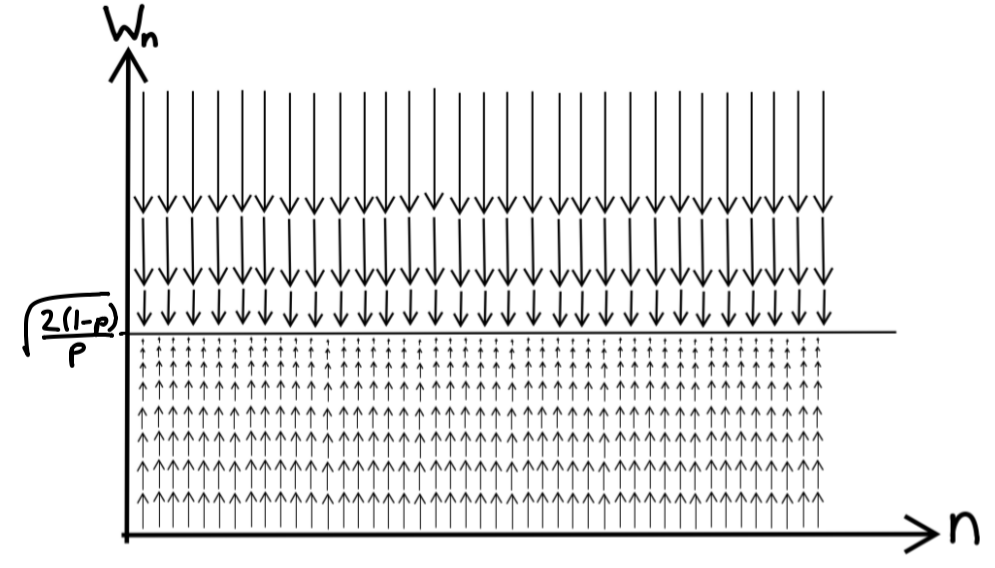
\includegraphics[width=0.6\textwidth]{./drift_chart_Wn}
\caption{Drift Model for $W_n$}
\end{figure}

\item We're given a sequence $(x_0, x_1, \dots, x_n)$ starting at $x_0 = 0$
and we decide to model it as a mean-reverting random walk as in question 5.
Explain how to estimate $\lambda$, $\mu$ and $\sigma$.

Using question 5:
\begin{align*}
\mathbb{E}(X_n) &= \mu
&
\text{Var}(X_n) &= \frac{\sigma^2}{1 - \lambda^2}
\end{align*}
\[
\begin{split}
\text{Var}(X_{n + 1} + X_n)
&= \text{Var}(\mu + \lambda(X_n - \mu) + \mathcal{N}(0, \sigma^2) + X_n) \\
&= \text{Var}((1 - \lambda)\mu + (\lambda + 1)X_n + \mathcal{N}(0,
\sigma^2)) \\
&= (\lambda + 1)\text{Var}(X_n) + \sigma^2 \\
&= \frac{(2 - \lambda)\sigma^2}{1 - \lambda} \\
\end{split}
\]

We now have an unbiased estimator for $\mu$ and can use fmin to find a
solution for $\mu$ and $\sigma$ for example by using the following code:
\begin{lstlisting}[language=Python, mathescape=true]
$\alpha$ = $\text{Var}(X_n)$
$\beta$ = $\text{Var}(X_{n+1} - X_n)$
def error(x):
	$\lambda$, $\sigma$ = x
	dif_$\alpha$ = $\alpha$ - $\frac{\sigma^2}{1 - \lambda^2}$
	dif_$\beta$ = $\beta$ - $\frac{(2 - \lambda)\sigma^2}{1 + \lambda}$
	return dif_$\alpha$ ** 2 + dif_$\beta$ ** 2
opt.fmin(error, [$\lambda_0$, $\sigma_0$])
\end{lstlisting}

\item Consider a moving object with noisy location readings. Let $X_n$ be
the location at timestep $n \geq 0$ and $Y_n$ the reading. Here's the
simulator.

\begin{lstlisting}[language=Python]
def hmm():
	max_state = 9
	x = np.random.randint(0, max_state + 1)
	while True:
		e = np.random.choice([-1, 0, 1])
		y = min(max_state, max(0, x + e))
		yield y
		d = np.random.choice([-1, 0, 1], p=[1/4, 1/2, 1/4])
		x = min(max_state, max(0, x + d))
\end{lstlisting}

We'd like to infer the location $X_n$ given readings $y_0, \dots y_n$.

\begin{enumerate}[label=(\alph*)]

\item Give justifications for the following three equations, which give an
inductive solution. First the base case,
\begin{align*}
\Pr(x_0 \ | \ y_0) &= c \times \Pr(x_0) \Pr(y_0 \ | \ x_0) \\
\intertext{and next two equations for the induction step,}
\Pr(x_n) &= \sum^{}_{x_{n-1}} \Pr(x_{n-1} \ | \ h) \Pr(x_n \ | \ x_{n-1}) \\
\Pr(x_n \ | \ h, y_n) &= c \times \Pr(x_n \ | \ h)\Pr(y_n \ | \ x_n)
\end{align*}

In these two equations, $h$ stands for $(y_0, \dots, y_{n-1})$ and we'll
assume we've already found $\Pr(x_{n-1} \ | \ h)$.

\begin{itemize}

\item $\Pr(x_0 \ | \ y_0) = c \times \Pr(x_0)\Pr(y_0 \ | \ x_0) $
\begin{align*}
\intertext{Using Bayes rule:}
\Pr(x_0 \ | \ y_0)
&= \frac{\Pr(x_0)\Pr(y_0 \ | \ x_0)}{\Pr(y_0)} \\
&= c \times \Pr(x_0) \Pr(y_0 \ | \ x_0) \\
\end{align*}

\item $\Pr(x_n) = \sum^{}_{x_{n-1}} \Pr(x_{n-1} \ | \ h) \Pr(x_n \ | \ x_{n-1}) \\$
\begin{align*}
\intertext{Using the law of total probability}
\Pr(x_n \ | \ h )
&= \sum_{x_{n-1}} \Pr(x_n, x_{n-1} \ | \ h) \\
&= \sum_{x_{n-1}} \Pr(x_{n-1} \ | \ h) \Pr(x_n \ | \
x_{n-1}, h) \\
\intertext{Since the next state depends only on the previous state}
&= \sum_{x_{n-1}} \Pr(x_{n-1} \ | \ h) \Pr(x_n \ | \ x_{n-1}) \\
\end{align*}

\item $\Pr(x_n \ | \ h, y_n) = c \times \Pr(x_n \ | \ h) \Pr(y_n \ | \ x_n) $

\begin{align*}
\Pr(x_n \ | \ h, y_n)
&= \frac{\Pr(y_n \ | \ x_n, h)\Pr(x_n \ | \ h)}{\Pr(y_n \ | \ h)} \\
&= c \times \Pr(y_n \ | \ x_n, h)\Pr(x_n \ | \ h) \\
\intertext{Since the observed state depends only on the hidden state}
&= c \times \Pr(y_n \ | \ x_n)\Pr(x_n \ | \ h) \\
\end{align*}

\end{itemize}

\item Give pseudocode for a function that takes as input a list of readings
$(y_0, \dots, y_n)$ and outputs the probability vector
\begin{align*}
& [\pi_0, \dots, \pi_{\text{MAX\_STATE}}]
&
\pi_x &= \mathbb{P}(X_n = x \ | \ y_0, \dots, y_n)
\end{align*}

\begin{lstlisting}[language=Python, mathescape=true]
def P($x_n$, $y_n$, h):
	$\pi$ = np.zeros(max_state)
	if $y_n$ = 0:
		$\pi$[0] = 2/3
		$\pi$[1] = 1/3
	elif $y_n$ = max_state:
		$\pi$[-1] = 2/3
		$\pi$[-2] = 1/3
	else:
		$\pi$[$y_n$-1:$y_n$+2] = 1/3
	if h.size == 0:
		return $\pi$
	for $x_n$ in states:
		$\pi$[$x_n$] *= np.sum(Pr($x_{n-1}$, h) * Pr_transition($x_{n-1}$, $x_n$))
	return $\pi$ / np.sum($\pi$)

def Pr_transition($x_{n-1}$, $x_n$):
	if $x_n$ == $x_{n-1}$:
		return 0.5
	elif abs($x_n$ - $x_{n-1}$) == 1:
		return 0.25
	else:
		return 0
\end{lstlisting}

\item If your code is given the input $(3, 3, 4, 9)$, it should fail with a
divide-by-zero error. Give an interpretation of this failure.

The observed dataset is impossible. The probability of the current
state being in any state is undefined; normalising undefined data is not
mathematically legal to do. So the code throws an exception.

\end{enumerate}

\end{enumerate}

\section{Supplementary Questions}

\begin{enumerate}

\setcounter{enumi}{9}

\item Here is the state space diagram for a Markov chain. Find a stationary
distribution. Is it unique?

\begin{center}
\begin{tikzpicture}
\node [state, place] (a) {$a$};
\node [state, place] (b) [right = of a] {$b$};
\path [->] (a) edge [loop left] node {$1 - \alpha$} ();
\path [->] (b) edge [loop right] node {$1 - \beta$} ();
\path [->] (a) edge [bend left] node[above] {$\alpha$} (b);
\path [->] (b) edge [bend left] node[below] {$\beta$} (a);
\end{tikzpicture}
\end{center}

With $\pi_x$ as the $x$ component of the stationary distribution, we can
form the equations:
\begin{align*}
\pi_a &= (1 - \alpha)\pi_a + \beta\pi_b
&
\pi_b &= \alpha \pi_a + (1 - \beta) \pi_b
&
1 &= \pi_a + \pi_b
\end{align*}

We can solve these to give the following values:

\begin{align*}
\pi_a &= \frac{\beta}{\alpha + \beta}
&
\pi_b &= \frac{\alpha}{\alpha + \beta}
\end{align*}

This stationary distribution is unique.

\item Here is the state space diagram for a Markov chain with state space
$\{0, 1, 2, \dots\}$. It is parameterized by $\alpha$ and $\beta$, with
$0 < \alpha < \beta$ and $\alpha + \beta < 1$. Let $\pi_n = \left( 1 -
\frac{\alpha}{\beta} \right)\left( \frac{\alpha}{\beta} \right)^n $, $n \geq
0$. Show that $\pi$ is a stationary distribution.

Firstly, we must prove that $\pi$ is a distribution:

\begin{align*}
\sum^{\infty}_{n=0} \pi_n
&= \sum^{\infty}_{n=0} \left(
\frac{\alpha}{\beta} \right)^n \\
&= \left( 1 - \frac{\alpha}{\beta} \right) \sum^{\infty}_{n=0} \left(
\frac{\alpha}{\beta} \right)^n \\
\intertext{Using the formula for the sum of a geometric distribution}
&= \left( 1 - \frac{\alpha}{\beta} \right) \frac{1}{1 -
\frac{\alpha}{\beta}} \\
&= 1 \\
\intertext{So $\pi$ is a valid distribution}
\end{align*}

To prove $\pi$ is a \textit{stationary} distribution, we must show that
$\mathbf{P}\pi = \pi$ where $\mathbf{P}$ is the transition matrix.
\begin{align*}
\intertext{For $n = 0$:}
\left(\mathbf{P}\pi\right)_n
&= \left( 1 - \alpha \right)\left( 1 - \frac{\alpha}{\beta} \right)\left(
\frac{\alpha}{\beta} \right)^n + \beta \left( 1 - \frac{\alpha}{\beta} \right)
\left( \frac{\alpha}{\beta} \right)^{n+1} \\
&= \left( 1 - \frac{\alpha}{\beta} \right)\left( \frac{\alpha}{\beta}
\right)^n\left( 1 - \alpha + \beta\frac{\alpha}{\beta} \right) \\
&= \left( 1 - \frac{\alpha}{\beta} \right)\left( \frac{\alpha}{\beta}
\right)^n\left( 1 - \alpha + \alpha \right) \\
&= \left( 1 - \frac{\alpha}{\beta} \right)\left( \frac{\alpha}{\beta}
\right)^n \\
&= \pi_n \\\\
\intertext{For $n \neq 0$:}
\left(\mathbf{P}\pi\right)_n
&= \sum^{\infty}_{i=0} \mathbf{P}_{n, i} \pi_i \\
&= \mathbf{P}_{n, n-1}\pi_{n-1} + \mathbf{P}_{n, n}\pi_n +
\mathbf{P}_{n, n+1} \pi_{n+1} \\
&= \alpha \left( 1 - \frac{\alpha}{\beta} \right)\left( \frac{\alpha}{\beta}
\right)^{n-1} + (1 - \alpha - \beta)\left( 1 - \frac{\alpha}{\beta} \right)
\left( \frac{\alpha}{\beta} \right)^n + \beta \left( 1 -
\frac{\alpha}{\beta} \right)\left( \frac{\alpha}{\beta}
\right)^{n+1} \\
&= \left( 1 - \frac{\alpha}{\beta} \right)\left( \frac{\alpha}{\beta}
\right)^n\left( \beta + 1 - \alpha - \beta + \alpha \right) \\
&= \left( 1 - \frac{\alpha}{\beta} \right)\left( \frac{\alpha}{\beta}
\right)^n \\
&= \pi_n \\
\end{align*}

\item Let $X_n \in \mathbb{N}$ be te number of infections people on day $n$
of an epidemic and consider the Markov chain model
\[
X_{n+1} = X_n + \mathbf{Po}\left(\frac{rX_n}{d}\right) - \mathbf{B}\left( X_n,
\frac{1}{d} \right)
\]

We would like to compute the probability that, starting from state $X_0 =
x$, the epidemic dies out i.e.\ hits state 0. In order to solve this by
computer, we'll cut the state space down to $\{0, \dots N\}$ for some
sufficiently large $N$ by amalgamating all the states with $\geq N$ infected
and letting the transition from state $N$ back to itself have probability 1.

\begin{enumerate}[label=(\alph*)]

\item Give pseudocode to compute the transition matrix. You should give your
answer in terms of \texttt{binom.pmf} and \texttt{poisson.pmf}, the
likelihood functions for the two distributions in question.

\begin{lstlisting}[language=Python, mathescape=true]
P = np.zeros((N, N))
for i in range(1, N-1):
	for j in range(N):
		prob = stats.poisson.pmf(j - i + np.arange(i+1), r * i / d) * \
		stats.binom.pmf(np.arange(i+1), i, 1 / d)
		P[i, j] = np.sum(prob)
P[0, 0] = 1
P[-1, -1] = 1
P /= np.sum(P, axis=1, keepdims=True)
\end{lstlisting}

\item Give pseudocode to compute the probability that the epidemic dies out, 
starting from any initial state $x \in \{0, \dots, N\}$.

\begin{lstlisting}[language=Python, mathescape=true]
condition1 = np.zeros(N)
condition1[0] = 1
condition2 = np.zeros(N)
condition2[-1] = 1
matrix = np.concatenate((P - np.eye(N), [condition1, condition2]))
print(matrix)
target = np.zeros(N + 2)
target[-2] = 1
np.linalg.lstsq(matrix, target, rcond=None)
\end{lstlisting}

\end{enumerate}

\item Consider a directed acyclic graph representing the web, with one
vertex per webpage and an edge $v \to w$ if page $v$ links to page $w$.
Consider a random web surfer who goes from page to page according to the
algorithm.

\begin{lstlisting}[language=Python, mathescape=true]
d = 0.85
def next_page($v$):
	neighbours = list of pages $w$ wuch that $v \to w$
	a = random.choice(['follow_link', 'teleport'], p=[d, 1-d])
	if a == 'follow_link' and len(neighbours) > 0:
		return random.choice(neighbours)
	else:
		$V$ = list of all web pages
		return random.choice($V$)
\end{lstlisting}

This solves a Markov chain. Explain why the chain is irreducible. Show that
the stationary distribution $\pi$ solves

\[
\pi_v = \frac{1 - d}{|V|} + d \sum^{}_{u:u \to v} \frac{\pi_u}{| \Gamma_u |}
\]

where $|V|$ is the total number of web pages in the graph and $|\Gamma_u|$ is
the number of outgoing edges from $u$.

Compute the stationary distribution for this random web surfer model, for the
graph in lecture notes example 10.3.1. Repeat with $d = 0.05$. What do you
expect as $d \to 0$? What do you expect if $d = 1$?

Irreducible means that there is a path from any state to any other state.
Since we can teleport from one state to any other state, we can clearly
reach any state from any other state.

The stationary distribution of the markov chain must maintain the invariant
that the probability of being in the state $v$ is the same as
the probability of being in the state $v$ after a step. Therefore:

\begin{align*}
\pi_v &= d\cdot \left(\mathbf{P}\pi\right)_v + \frac{1 - d}{|V|} \\
\pi_v &= \frac{1 - d}{|V|} + d\sum_{u:u\to v} \frac{\pi_u}{|\Gamma_u|}
\intertext{As required}
\end{align*}

\begin{lstlisting}[language=Python]
edges = np.array([
    [0, 1, 1, 0, 0, 0],
    [1, 0, 0, 0, 1, 1],
    [0, 1, 0, 1, 0, 0],
    [0, 0, 1, 0, 1, 1],
    [0, 0, 0, 1, 0, 0],
    [0, 0, 0, 0, 0, 1]
])
n = edges.shape[0]
P = edges / np.sum(edges, axis=1, keepdims=True)
P *= d
P += (1 - d) / n
matrix = np.concatenate((P.transpose() - np.eye(n), [np.ones(n)]))
np.linalg.lstsq(matrix, [0, 0, 0, 0, 0, 0, 1], rcond=None)
\end{lstlisting}

For $d = 0.85$ this returns:
\[
\pi =
\begin{pmatrix}
0.047839\\
0.080608\\
0.083004\\
0.132961\\
0.085511\\
0.570076\\
\end{pmatrix}
\]

For $d = 0.05$ this returns:
\[
\pi =
\begin{pmatrix}
0.161108\\
0.166491\\
0.165205\\
0.170661\\
0.163953\\
0.172582\\
\end{pmatrix}
\]

As $d \to 0$, the distribution will tend to $\pi = (0, 0, 0, 0, 0, 1)$. If
$d = 1$ then the distribution $\pi$ is $\left( \frac{1}{6}, \frac{1}{6},
\frac{1}{6}, \frac{1}{6}, \frac{1}{6}, \frac{1}{6} \right)$.

\item Consider the random web surfer model for the graph in lecture notes
example 10.3.1. Let $t_x$ be the expected time, starting from vector $x$
until the server reaches vertex 5. Derive the equations:
\[
t_x = 1 + \sum^{}_{y} P_{xy}t_y \ \ \ \text{for all x $\neq$ 5,} \ \ \ t_5
= 0
\]

and solve with numpy

\begin{lstlisting}[language=Python]
edges = np.array([
    [0, 1, 1, 0, 0, 0],
    [1, 0, 0, 0, 1, 1],
    [0, 1, 0, 1, 0, 0],
    [0, 0, 1, 0, 1, 1],
    [0, 0, 0, 1, 0, 0],
    [0, 0, 0, 0, 0, 1]
])
n = edges.shape[0]
P = edges / np.sum(edges, axis=1, keepdims=True)
P -= np.eye(n)
P = np.concatenate((P, [[0, 0, 0, 0, 0, 1]]))
np.linalg.lstsq(P, [-1, -1, -1, -1, -1, 0, 0], rcond=None)
\end{lstlisting}

The result is:
\[
\begin{pmatrix}
6.73 \\
5.27 \\
6.18 \\
5.09 \\
6.09 \\
0.00 \\
\end{pmatrix}
\]

\item The code from question 8(c) can fail with a divide-by-zero error.
This is undesirable in production code! One way to fix the problem is ot
modify the Markov model to include a ``random teleport'' -- to express the
idea ``Okay, our interface has gone wrong somewhere; let's allow our
location estimate to reset itself''. We can achieve this mathematically with
the following model: with probability $1 - \varepsilon$ generate the next
state as per line 9, otherwise pick the next state uniformly from $\{0, 1,
\dots, \text{MAX\_STATE}\}$. Modify your code from question $b$ to reflect
this new model with $\varepsilon = 0.01$.

The only changes necessary are to the function \texttt{Pr\_transition}:

\begin{lstlisting}[language=Python, mathescape=true]
def Pr_transition($x_{n-1}$, $x_n$):
	if $x_n$ == $x_{n-1}$:
		p = 0.5
	elif abs($x_n$ - $x_{n-1}$) == 1:
		p = 0.25
	else:
		p = 0
	p *= (1 - $\varepsilon$)
	p += $\varepsilon$ / (max_state + 1)
	return p
\end{lstlisting}

Alternatively, we could fix the problem by changing the model to express
``Okay, this reading is glitchy; let's allow the code to discard an
impossible reading''. How might you change the Markov model to achieve this?

We can give all states an infinitesimally small probability $\delta$ of
emitting a random observation. With $\delta$ small enough, an impossible
observation becomes an unknown observation while $\delta$ will not
meaningfully affect the probabilities of known observations. If there is a
known probability of a glitchy reading, we may want to have a non-negligible
probability.

\item The Markov Model for motion from question 1 is called a \textit{simple
random walk (\textit{with boundaries})}; it chooses a direction fo travel
independently at every timestep. This is not a good model for human
movement, since people tend to head in the same direction for a while
before changing direction.

\begin{enumerate}[label=(\alph*)]

\item Let $V_n \in \{-1, 0, 1\}$ be a Markov chain: let $V_{n+1} = V_n$ with
probability 0.9, and let $V_{n+1}$ be chosen uniformly at random from $\{-1,
0, 1\}$ with probability 0.1. Draw a state space diagram for this Markov chain.

\begin{center}
\begin{tikzpicture}

\node [state, place2] (v0) {$V_0$};
\node [state, place2] (v-1) [at=(v0), shift=(240:3.5cm)]
{$V_{-1}$};
\node [state, place2] (v1) [at=(v0), shift=(300:3.5cm)] {$V_1$};

\path [->] (v0) edge [bend left, out=10, in=170]
node[anchor=210] {$\frac{1}{30}$} (v1);
\path [->] (v0) edge [bend left, out=10, in=170]
node[anchor=150]{$\frac{1}{30}$} (v-1);

\path [->] (v1) edge [bend left, out=10, in=170] node[anchor=30]
{$\frac{1}{30}$} (v0);
\path [->] (v1) edge [bend left, out=10, in=170] node[anchor=90]
{$\frac{1}{30}$}
(v-1);

\path [->] (v-1) edge [bend left, out=10, in=170] node[anchor=-30]
{$\frac{1}{30}$} (v0);
\path [->] (v-1) edge [bend left, out=10, in=170] node[anchor=270]
{$\frac{1}{30}$}(v1);

\path (v0) edge [loop above] node[above] {$\frac{14}{15}$} ();
\path (v1) edge [loop right] node[right] {$\frac{14}{15}$} ();
\path (v-1) edge [loop left] node[left] {$\frac{14}{15}$} ();

\end{tikzpicture}
\end{center}

\item Interpret $V_n$ as the velocity of our moving object at timestep $n$,
and let $X_{n+1} = \max\left(0, \min\left(9, X_n + V_n\right)\right)$.

Draw the state space diagram for $(X_n, V_n)$.

For brevity, normal lines have probability $\frac{1}{30}$ and thick lines
have probability $\frac{14}{15}$. I have only drawn the first four $X_i$ due
to space constraints.

\begin{center}
\begin{tikzpicture}
\node (x0v0) {$X_0, V_0$};
\node (x0v1) [above = of x0v0] {$X_0, V_1$};
\node (x0v-1) [below = of x0v0] {$X_0, V_{-1}$};
\node (x1v0) [right = 2cm of x0v0] {$X_1, V_0$};
\node (x1v1) [above = of x1v0] {$X_1, V_1$};
\node (x1v-1) [below = of x1v0] {$X_1, V_{-1}$};
\node (x2v0) [right = 2cm of x1v0] {$X_2, V_0$};
\node (x2v1) [above = of x2v0] {$X_2, V_1$};
\node (x2v-1) [below = of x2v0] {$X_2, V_{-1}$};
\node (x3v0) [right = 2cm of x2v0] {$X_3, V_0$};
\node (x3v1) [above = of x3v0] {$X_3, V_1$};
\node (x3v-1) [below = of x3v0] {$X_3, V_{-1}$};

\path [->, line width=1.2pt] (x0v1) edge [bend left, out=10, in=170] (x1v1);
\path [->, line width=1.2pt] (x1v1) edge [bend left, out=10, in=170] (x2v1);
\path [->, line width=1.2pt] (x2v1) edge [bend left, out=10, in=170] (x3v1);

\path [->, line width=1.2pt] (x1v-1) edge [bend left, out=10, in=170] (x0v-1);
\path [->, line width=1.2pt] (x2v-1) edge [bend left, out=10, in=170] (x1v-1);
\path [->, line width=1.2pt] (x3v-1) edge [bend left, out=10, in=170] (x2v-1);

\path [->, line width=1.2pt] (x0v0) edge [loop left] ();
\path [->, line width=1.2pt] (x1v0) edge [loop left] ();
\path [->, line width=1.2pt] (x2v0) edge [loop left] ();
\path [->, line width=1.2pt] (x3v0) edge [loop left] ();

\path [->] (x0v-1) edge [bend left, out=10, in=170] (x0v0);
\path [->] (x1v-1) edge [bend left, out=10, in=170](x1v0);
\path [->] (x2v-1) edge [bend left, out=10, in=170] (x2v0);
\path [->] (x3v-1) edge [bend left, out=10, in=170] (x3v0);

\path [->] (x0v1) edge [bend left, out=10, in=170]  (x0v0);
\path [->] (x1v1) edge [bend left, out=10, in=170]  (x1v0);
\path [->] (x2v1) edge [bend left, out=10, in=170] (x2v0);
\path [->] (x3v1) edge [bend left, out=10, in=170] (x3v0);

\path [->, line width=1.2pt] (x0v-1) edge [loop left] (x0v-1);

\path [->] (x0v1) edge [bend left] (x0v-1);
\path [->] (x1v1) edge [bend left] (x0v-1);
\path [->] (x2v1) edge [bend left] (x1v-1);
\path [->] (x3v1) edge [bend left] (x2v-1);

\path [->] (x0v-1) edge [bend left] (x1v1);
\path [->] (x1v-1) edge [bend left] (x2v1);
\path [->] (x2v-1) edge [bend left] (x3v1);

\end{tikzpicture}
\end{center}

\item Give pseudocode to compute the stationary distribution.

\begin{lstlisting}[language=Python]
probs = np.zeros((30, 30))
#  0-9 is x0v-1 - x9v-1
# 10-19 is x0v-1 - x9v-1
# 20-29 is x0v-1 - x9v-1
probs[np.arange(1, 10), np.arange(9)] = 14/15
probs[0, 0] = 14/15
probs[np.arange(10), np.arange(10, 20)] = 1/30
probs[np.arange(9), np.arange(21, 30)] = 1/30
probs[9, 29] = 1/30

probs[np.arange(10, 20), np.arange(10, 20)] = 14/15
probs[np.arange(11, 20), np.arange(0, 9)] = 1/30
probs[10, 0] = 1/30
probs[np.arange(10, 19), np.arange(21, 30)] = 1/30
probs[19, 29] = 1/30

probs[np.arange(20, 29), np.arange(21, 30)] = 14/15
probs[29, 29] = 14/15
probs[np.arange(20, 30), np.arange(10, 20)] = 1/30
probs[np.arange(21, 30), np.arange(9)] = 1/30
probs[20, 0] = 1/30

mat = np.concatenate((probs.transpose() - np.eye(30), np.ones((1, 30))))

target = np.zeros(31)
target[30] = 1

np.linalg.lstsq(mat, target, rcond=None)
\end{lstlisting}

\end{enumerate}

\end{enumerate}

\begin{examquestion}{2020}{6}{7}

Consider the probability model

\begin{center}
\begin{tikzpicture}
\node (x0) {$X_0$};
\node (x1) [right = of x0] {$X_1$};
\node (x2) [right = of x1] {$X_2$};
\node (x3) [right = of x2] {$X_3$};
\node (dot) [right = of x3] {\ldots};
\node (y1) [below = of x1] {$Y_1$};
\node (y2) [below = of x2] {$Y_2$};
\node (y3) [below = of x3] {$Y_3$};
\path [->] (x0) edge (x1);
\path [->] (x1) edge (x2);
\path [->] (x2) edge (x3);
\path [->] (x3) edge (dot);
\path [->] (x1) edge (y1);
\path [->] (x2) edge (y2);
\path [->] (x3) edge (y3);
\end{tikzpicture}
\end{center}

where $(X_0, X_0, \dots)$ is a Markov chain on state space $\{0, 1\}$ with
transition probabilities $P_{01} = p$, $P_{10} = q$; and where each $Y_i$ is
normally distributed with mean $X_i$ and variance $\sigma^2$.

We are given a sequence of obserations $(y_1, y_2, \dots, y_n)$, and we wish
to make an inference about the unobserved values $(X_1, X_2, \dots, X_n)$.
We will take $0 < p < 1$, $0 < q < 1$ and $\sigma > 0$ to be known and we
will assume that $X_0$ is sampled from the Markov Chain's stationary
distribution.

\begin{enumerate}[label=(\alph*)]

\item Write out the transition matrix for the Markov Chain $(X_0, X_1,
\dots)$. Calculate its stationary distribution.

With $\mathbf{P}$ as the transition matrix for the Matrix Chain:

\[
\mathbf{P} =
\begin{pmatrix}
1 - p & p \\
q & 1 - q \\
\end{pmatrix}
\]

The stationary distribution $\pi$ satisfies $\mathbf{P}\pi = \pi$. Therefore:

\begin{align*}
(1 - p)\pi_0 + q\pi_1 &= \pi_0 & p\pi_0 + (1 - q)\pi_1 &= \pi_1 & \pi_0 +
\pi_1 &= 1 \\
q\pi_1 - p\pi_0 &= 0 & p\pi_0 - q\pi_1 &= 0 & \pi_0 + \pi_1 &= 1 \\
q\pi_1 - p(1 - \pi_1) &= 0 \\
(p + q)\pi_1 &= p \\
\pi_1 &= \frac{p}{p + q} \\
\end{align*}

Therefore:
\begin{align*}
\pi_0 &= \frac{q}{p + q} & \pi_1 &= \frac{p}{p + q} \\
\end{align*}

\item Writing $\overrightarrow{X}$ for $(X_0, X_1, \dots, X_n)$ and writing
$ \overrightarrow{Y} $ for $(Y_1, \dots, Y_n)$ and similarly $ \overrightarrow{x} $
and $ \overrightarrow{y} $, find expressions for:

\[
\mathbb{P}( \overrightarrow{X} = \overrightarrow{x} ) \ \ \text{and for} \ \
\mathbb{P}( \overrightarrow{Y} = \overrightarrow{y} \ | \ \overrightarrow{X}
 = \overrightarrow{x} )
\]

I will use list slicing notation $[:i]$ to mean ``the first $i$ values''.
For example $ \overrightarrow{x}[:2] $ means $x_0, x_1$.

\[
\begin{split}
\mathbb{P}( \overrightarrow{X} = \overrightarrow{x} ) &=
\mathbb{P}(x_0) \cdot \mathbb{P}(x_1 \ | \ \overrightarrow{x}[:1] ) \cdot
\dots \cdot \mathbb{P}(x_n \ | \ \overrightarrow{x}[:n] ) \\
\intertext{Using Memorylessness:}
\mathbb{P}( \overrightarrow{X} = \overrightarrow{x} ) &=
\mathbb{P}(x_0) \cdot \mathbb{P}(x_1 \ | \ x_0 ) \cdot
\dots \cdot \mathbb{P}(x_n \ | \ x_{n-1} ) \\
&= \pi_{x_0} \cdot \prod^{n-1}_{i=0} \mathbf{P}_{X_i X_{i+1}} \\
\end{split}
\]

Since the observed value of a Markov Chain depends only on its current state:

\[
\begin{split}
\mathbb{P}( \overrightarrow{Y} = \overrightarrow{y} \ | \ \overrightarrow{X}
= \overrightarrow{x} )
&= \prod^{n}_{i=1} \Pr(y_i \ | \ x_i) \\
&= \prod^{n}_{i=1} \frac{1}{\sqrt{2\pi} \sigma} e^{-\frac{(y_i - x_i)^2
}{2\sigma^2}} \\
&= \left(\frac{1}{\sqrt{2\pi} \sigma}\right)^n e^{-\frac{\sum^n_{i=1}(y_i -
x_i)^2
}{2\sigma^2}} \\
\end{split}
\]

\item Give pseudocode for a function \texttt{rx(n)} that generates a random
$ \overrightarrow{X} $. Give pseudocode to generate a weighted sample from
the posterior distribution of $ \overrightarrow{X} $ conditional on the
observed data $ \overrightarrow{Y} = \overrightarrow{y} $.

\begin{lstlisting}[language=Python, mathescape=true]
def rx(n):
	x = np.random.choice(2, 1, $\pi$)
	for i in range(n):
		x.append(np.random.choice(2, p=$\pi$[x[-1]]))
	return x
\end{lstlisting}

We can generate a weighted sample by randomly generating samples
$\overrightarrow{x}$ using \texttt{rx(n)} and sampling using
$ \mathbb{P}( \overrightarrow{y} \ | \ \overrightarrow{x} ) $ as the weight.

\begin{lstlisting}[language=Python, mathescape=true]
def P(x, y):
	# work out $\mathbb{P}( \overrightarrow{y} \ | \ \overrightarrow{x} )$
	p = [$\frac{1}{\sqrt{2\pi}\sigma} \cdot e^{-\frac{(y_i - x_i)^2}{2\sigma^2}}$ for $x_i$, $y_i$ in zip(x, y)]
	prob = 1
	for $p_i$ in p:
		prob *= $p_i$
	return prob

def weighted_rx(y, samples=1000):
	samples = [rx(len(y)) for _ in range(samples)]
	probs = [P($\overrightarrow{x}$, y) for $\overrightarrow{x}$ in samples]
	return samples[np.random.choice(samples + 1, p=probs / sum(probs))]
\end{lstlisting}

\item Let $Z = \frac{\sum^n_{i=1}X_i}{n}$. Give pseudocode to find a $95\%$
confidence interval for $Z$, conditional on the observed data
$ \overrightarrow{Y} = \overrightarrow{y} $.

\begin{lstlisting}[language=Python, mathescape=true]
lo = 0.025
hi = 0.975
$\overrightarrow{x}s$ = [weighted_rx($\overrightarrow{y}$) for _ in range(1000)]
zs = np.mean($\overrightarrow{x}s$[:, 1:], axis=1)
np.quantile(zs, [lo, hi])
\end{lstlisting}

\end{enumerate}

\end{examquestion}

\begin{examquestion}{2022}{6}{8}

Let $(E_0, E_1, \dots)$ be a Markov Chain generated by

\[
E_{t+1} = \lambda E_i + \mathcal{N}(0, (1 - \lambda^2)\sigma^2)
\]

where $0 \leq \lambda < 1$

\begin{enumerate}[label=(\alph*)]

\item What is meant by a stationary distribution?

A stationary distribution is a probability vector $\pi$ such that the
probability of being in state $i$ at time $t$ is equal to $\pi_i$ for all $t$.

\item What is meant by ``memorylessness''? Give an expression for the log
likelihood of a sequence of values $(e_1, \dots, e_n)$ given the value for
$E_0$.

Memorylessness means that the future state and observations from a Markov
Chain are dependent only on the current state. AKA the current state
contains all the information about the system.

\[
\ln\Pr(e_n\dots e_1 \ | \ E_0) = \ln\Pr(e_1 \ | \ E_0) + \sum^{n}_{i=2}\ln\Pr
(e_{i} \ | \ e_{i-1})
\]

\end{enumerate}

Klaus Hasselmann, who won the 2021 Nobel Prize, studied climate models in
which short-term random fluctuations can have longer-term effects. Suppose
we're given a dataset $(y_0, y_1, \dots, y_n)$ of temperatures at timepoints
$t = 0, 1, \dots n$, and we use a Hasselmann-style model,

\[
Y_t = \alpha + \beta \sin(2\pi \omega t) + \gamma t + E_t
\]

where $(E_0, E_1, \dots)$ is a Markov Chain as described above, and
$\alpha$, $\beta$ and $\gamma$ are unknown parameters to be estimated.

\begin{enumerate}[label=(\alph*)]

\setcounter{enumi}{2}

\item Give an expression for the log likelihood of $(y_1, \dots, y_n)$, given
the value for $Y_0$.

\begin{align*}
\Pr(Y_{t+1} \ | \ Y_t)
&= \Pr(E_{t+1} = Y_{t+1} - \alpha - \beta\sin(2\pi\omega(t+1)) - \gamma(t +
 1) \ | \ E_t = Y_t - \alpha - \beta\sin(2\pi\omega(t)) - \gamma t) \\
&= \frac{1}{\sqrt{2\pi}(1 - \lambda)\sigma}e^{-\frac{
(Y_{t+1} - Y_t - \beta\sin(2\pi\omega(t+1)) - \beta\sin(2\pi\omega t) -
\gamma)^2}{2(1 - \lambda)^2\sigma^2}} \\
\intertext{Using memorylessness:}
\Pr(y_1,\dots, y_n \ | \ Y_0)
&= \Pr(y_1 \ | \ Y_0) \cdot \prod^{n-1}_{t=1} \Pr(y_{t+1} \ | \ y_t) \\
\intertext{Therefore the log likelihood is given by:}
\ln\Pr(y_1,\dots, y_n \ | \ Y_0) &=
\ln\Pr(y_1 \ | \ Y_0) + \sum^{n-1}_{t=1} \ln\Pr(y_{t+1} \ | \ y_t) \\
&=
-\frac{n}{2}\ln(2\pi) - n\ln\sigma - \frac{(y_0 - Y_0 - \beta\sin2\pi\omega
 - \gamma)^2}{2(1 - \lambda)^2\sigma^2} \\ & - \sum^{n-1}_{t=1} \frac{
 (y_{t+1} - y_t - \beta\sin(2\pi\omega(t+1)) - \beta\sin
 (2\pi\omega t) - \gamma)^2}{2(1 - \lambda)^2\sigma^2}
\end{align*}

\item What is meant by a ``linear model''? Write out a linear model that can
be used to estimate the unknown parameters $\alpha$, $\beta$ and $\gamma$
(treating all other parameters as known). Identify the feature vectors.

A linear model is a model which only has linear coefficients. IE the model
is a linear combination of the feature vectors. The feature vectors
themselves may be nonlinear functions, however the unknown parameters can be
represented as a matrix equation.

\begin{align*}
\forall t \in \mathbb{N}. \mathbb{E}(E_t) &= 0 \\
\intertext{We can use this to write a formula for the expectation of $Y_t$:}
\mathbb{E}(Y_t) &= \alpha + \beta\sin(2\pi\omega t) + \gamma t \\
\end{align*}

We can now rerun the experiment many times and average this to approximate
the mean for $Y_0$, $Y_1$ and $Y_2$. Using the Central Limit Theorem, our
estimates will tend towards the true values.

Using the above formula $\mathbb{E}(Y_0) = \alpha$. Therefore we can
get an unbiased maximum likelihood estimator for $\alpha$ by averaging many
$Y_0$.

We can form equations for $Y_1$ and $Y_2$ which we can use to give
estimators for $\beta$ and $\gamma$:

\begin{align*}
\mathbb{E}(Y_1) &= \alpha + \beta\sin(2\pi\omega) + \gamma & \mathbb{E}
(Y_2) &= \alpha + \beta\sin(4\pi\omega) + 2\gamma \\
\end{align*}

These can be rearranged into a matrix equation:
\[
\begin{split}
\begin{pmatrix}
\sin(2\pi\omega) & 1 \\
\sin(4\pi\omega) & 2 \\
\end{pmatrix}
\begin{pmatrix}
\beta \\ \gamma \\
\end{pmatrix}
&=
\begin{pmatrix}
\mathbb{E}(Y_1) - \alpha \\
 \mathbb{E}(Y_2) - \alpha \\
\end{pmatrix} \\
\begin{pmatrix}
\beta \\ \gamma \\
\end{pmatrix}
&=
\frac{1}{2\sin(2\pi\omega) - \sin(4\pi\omega)}
\begin{pmatrix}
2 & -1 \\
-\sin(4\pi\omega) & \sin(2\pi\omega) \\
\end{pmatrix}
\begin{pmatrix}
\mathbb{E}(Y_1) - \alpha \\
 \mathbb{E}(Y_2) - \alpha \\
\end{pmatrix} \\
\end{split}
\]

\end{enumerate}

\end{examquestion}

\end{document}
